
\chapter{Introduction}


\section{Problem Background}
\label{sec:chap1-problem}


%- first paragraph: convince it's super important problem. why perimain basin matters, and what's the problem
%- have wells, inducsed seismicity, rate hasskyrocket, mention one year has more than CA.
%- also btw, this is difficult. not all wells induce. some wells opearate fine, no issues, some wells have delayed, and keep having EQs about stop.
%- even people without background should find intersting, even without texas background.
%- people in general like to hear problems, and where people are stuck, and why they care to work on.
%- Natl academy science report shold have highlights to take.
%- ESI proposal: use from that

The Permian Basin, stretching from eastern New Mexico and covering most of West Texas, has become the United States' largest producer of oil and gas over the past decade (Figure \ref{fig:permian-overview}a). The region's production began to take off around 2009, largely due to advances in horizontal drilling and multi-stage hydraulic fracturing.
The rapid expansion of oil and gas production from shale formations has created positive economic impacts as well as sociopolitical concerns, given that researchers have long recognized that injection or withdrawal of fluids from the subsurface can induce earthquakes along existing faults \citep{Council2013InducedSeismicityPotential, Simpson1988TwoTypesReservoir, Ellsworth2013InjectionInducedEarthquakes}. Similar to other oil production and wastewater injection sites around the world (e.g. the central and eastern United States, Canada, China, and Italy) \citep{Foulger2018GlobalReviewHuman}, the Permian Basin has experienced a dramatically increased rate of low magnitude earthquakes over the past decade \citep{Frohlich2016HistoricalReviewInduced, Atkinson2016HydraulicFracturingSeismicity, Frohlich2019OnsetCauseIncreased, Lomax2019ImprovingAbsoluteEarthquake, Savvaidis2020InducedSeismicityDelaware, Skoumal2020InducedSeismicityDelaware} (Figure \ref{fig:permian-overview}b). For example, Texas recorded over 200 magnitude 3.0 or greater earthquakes in 2021, second only to California in the contiguous United States.  While petroleum production and wastewater injection volumes have been rising throughout the basin, the recently cataloged earthquakes are spatially clustered. In order to assess the damage potential from induced and triggered earthquakes, we need to acquire new data and develop new monitoring approaches to better understand which earthquakes are induced, which wells they are associated with, and why some high rate wells experience seismicity while others do not. 

\begin{figure}
	\centering
	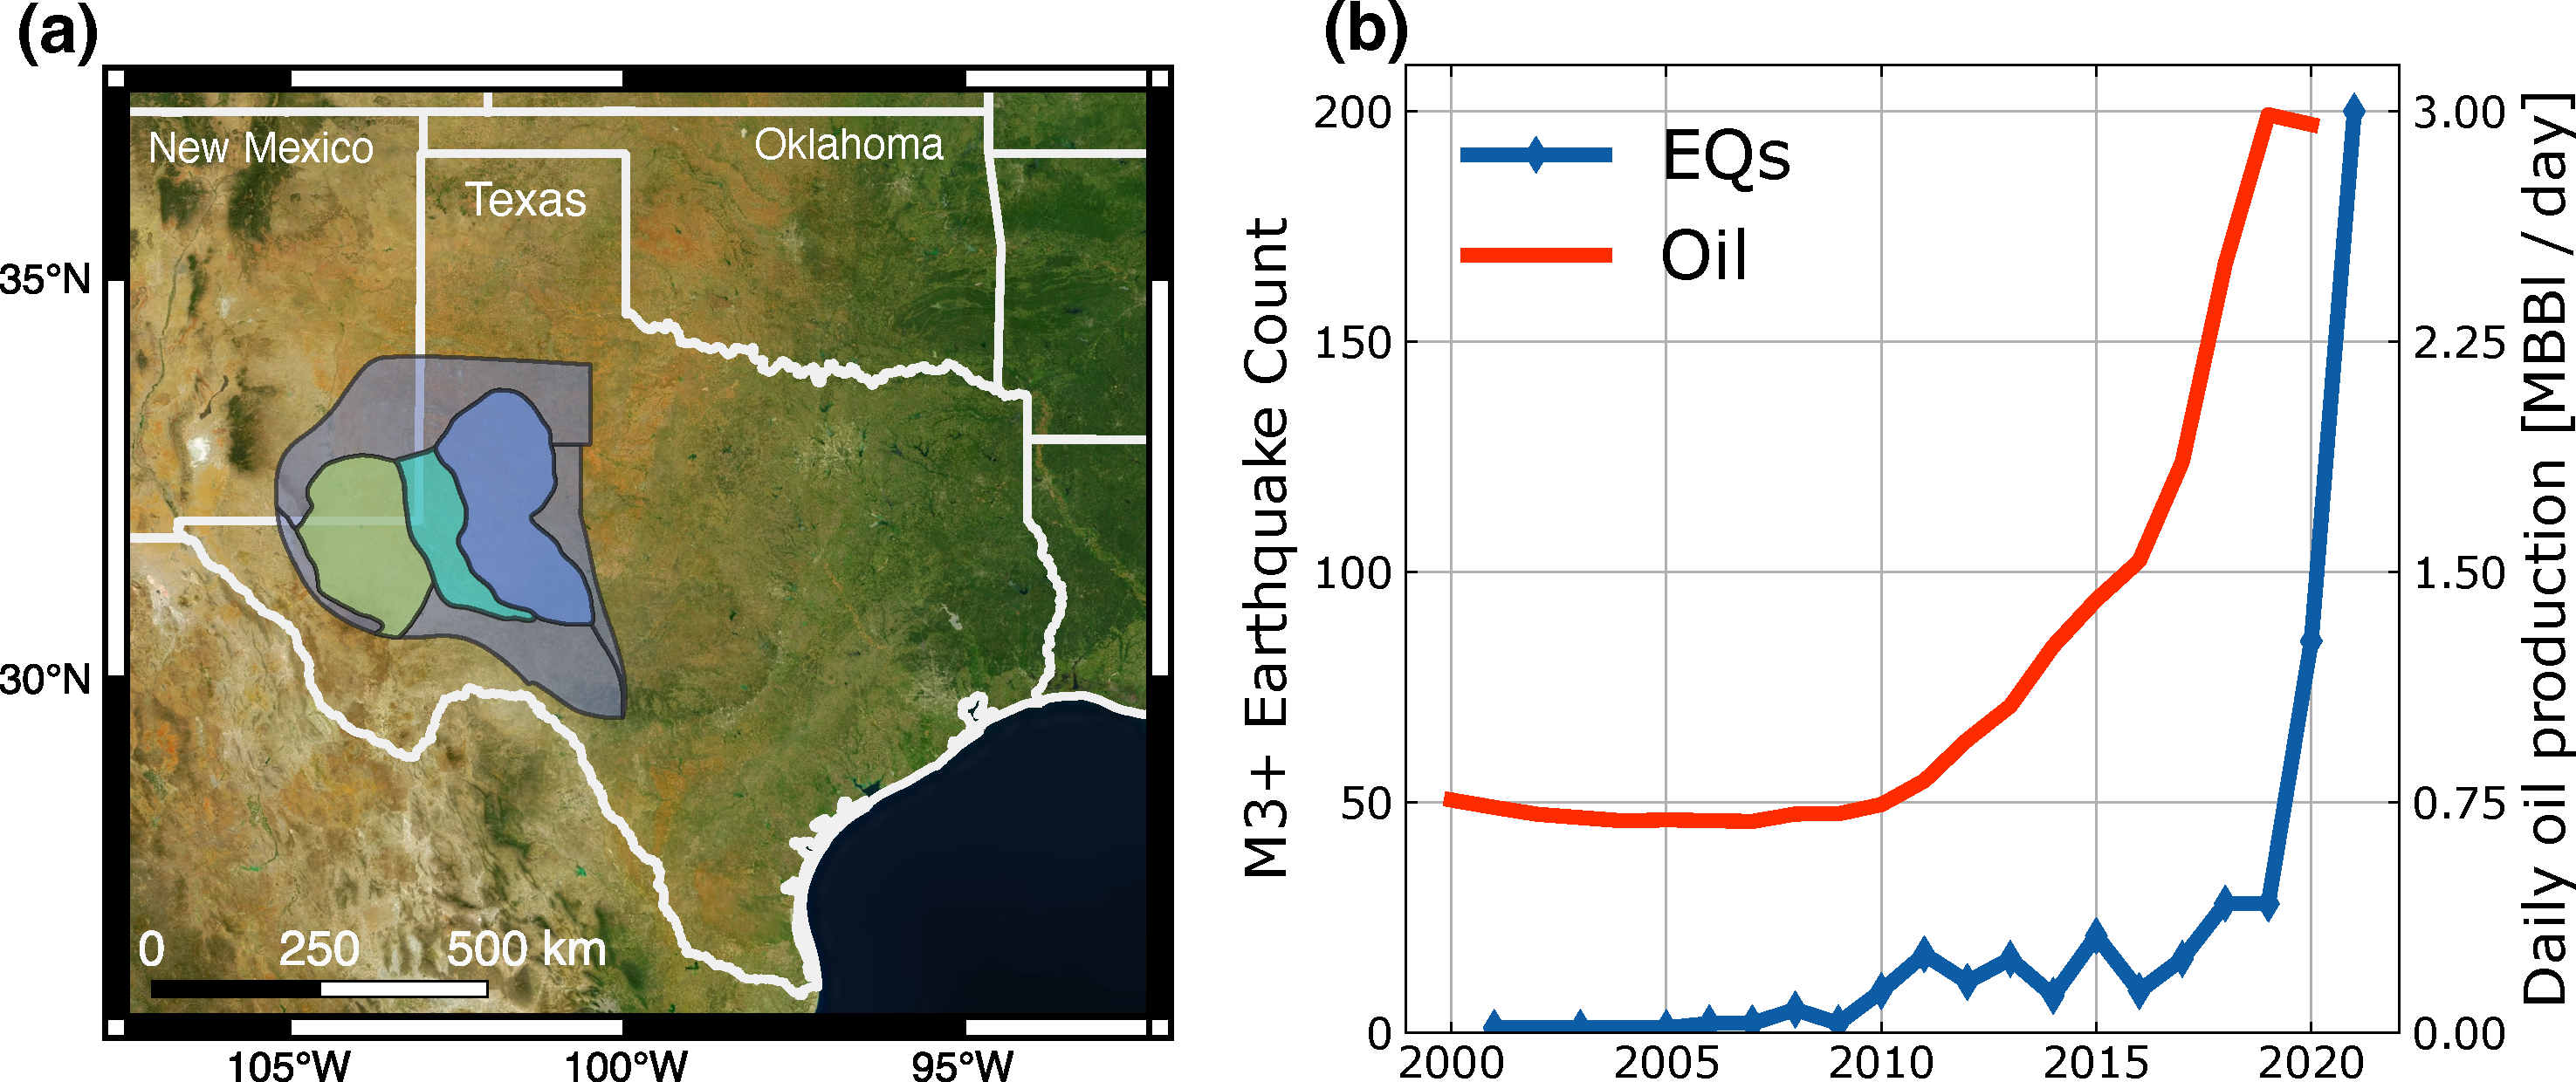
\includegraphics[width=\columnwidth]{figures/permian-overview-eqs-oil.pdf}
	\caption[Permian Basin oil production and earthquakes]{
		(a) Location of Permian Basin within Texas. The subbasins colored within the Permian Basin are (from west to east) the Delaware Basin (green), Central Basin Platform (cyan), and Midland Basin (purple).
		(b) Yearly number of magnitude 3 or larger earthquakes recorded within Texas since 2000 (blue line), and average daily oil production per year for Permian Basin wells in Texas (red line).
		Earthquakes retrieved from USGS at \url{https://earthquake.usgs.gov} . Oil Production data retrieved from the Texas Railroad Commission's production query system at \url{https://www.rrc.texas.gov} .
	}
	\label{fig:permian-overview}
\end{figure}

%After you bring it up it is hard to collect in-situ measurements. You may first mention there is a large volume of spaceborne InSAR data, and then explain why InSAR is useful for the West Texas problem. Then you should review relevant InSAR work in West Texas, and bring up the challenge of large scale processing (1. tropospheric noise increases over distance 2. the noise magnitude can be ~ 10 cm or more). 
%At minimum, we should include all discussion in the GRL/TGRS introduction, but perhaps we need a little more so that chapter 5 is also covered under this review.



%One significant cluster is near Pecos, TX, where increased seismic activity began in 2009 and climbed to more than 2000 earthquakes in 2017 \citep{Frohlich2019OnsetCauseIncreased}. Unfortunately, detailed in-situ measurements of the subsurface can be costly or infeasible to perform across the $\sim$200,000 km$^2$ Permian Basin.

In 2017, the State of Texas funded a state-wide seismicity monitoring system known as TexNet, which enables the cataloging of earthquakes across Texas at magnitudes down to about M2.0 \citep{Savvaidis2019TexnetStatewideSeismological}. However, it is difficult to examine the mechanism, scale, scope, and consequences of induced seismicity in the geologically-complex Permian Basin. This is because (1) in-situ measurements of the earth's subsurface (e.g the fault geometries and characteristics of the petroleum reservoirs) are extremely limited; and (2) systematic and sustained collection of such data across the $\sim$200,000 km$^2$ Basin represents a costly undertaking with significant technical uncertainties \citep{Hennings2021StabilityFaultSystems}.


Since the launch of the Sentinel-1 mission in 2014, the quantity and quality of open-access Interferometric Synthetic Aperture Radar (SAR) data has grown exponentially. InSAR techniques can measure millimeter-to-centimeter deformation of Earth's surface over very wide areas with 10s-to-100s meter spatial resolution \citep{Massonnet1993DisplacementFieldLanders, Buergmann2000SyntheticApertureRadar}. These high-quality surface deformation measurements can be used to locate previously unknown faults, estimate the distribution of fault slip, and infer associated seismic risk at very low cost \citep{Segall2010EarthquakeVolcanoDeformation, Elliott2016RoleSpaceBased, Huang2017FaultGeometryInversion}. \cite{Shirzaei2016SurfaceUpliftTime} reported indications of surface uplift due to wastewater injection near a 2012 M4.8 Timpson earthquake site, though limited validation for the InSAR results was available \citep{Semple2017IncompleteInventorySuspected}.
\cite{Kim2018AssociationLocalizedGeohazards} detected multiple deformation bowls within the Delaware Basin related to wastewater injection, $CO_2$ injection, and hydrocarbon production using Sentinel-1 InSAR data. \cite{Zheng2019WastewaterLeakageWest} incorporated InSAR-derived surface deformation data into a poroelastic model to analyze the geomechanical processes near an uplift signal in northern West Texas. They discovered that the observed surface deformation was likely caused by injection well leakages, rather than pressure increases at the planned injection depth, and the leaks may have contributed to freshwater contamination. More recently, \cite{Deng2020SurfaceDeformationInduced} used ascending Sentinel-1 LOS measurements to infer pore pressure change and Coulomb failure stress change at three sites in the southern Delaware Basin. They suggested that certain groups of earthquakes are likely induced by fluid injection, but noted that local rock structure and media properties are key controls on the area's susceptibility to induced seismicity.


%%ANN: This leads to a review of the current methods for characterizing or mitigating tropospheric noise, and some limitations. %The review of previous work on tropospheric noise characteristics/mitigations in chapter 1 does not need to be very specific (as we have a detailed review later, and we do not need to introduce unnecessary repetitions), but I think it is important to summarize the general approach and the limitations (with key references).

The existing studies mainly focused on sites $ \sim $ 60-by-60 $km^2$ or smaller, but basin-wide InSAR surface deformation data with detailed uncertainty quantification are needed for assessing regional induced seismicity risk. 
One of the challenges for large- is noise arising from changes in water vapor content within the troposphere.
Tropospheric noise varies substantially in both space and time, and the noise variance grows with the size of the study area (occasionally reaching 10-20 cm).
Previous studies have developed empirical correction techniques \citep{Lauknes2011InsarTroposphericStratification, Bekaert2015SpatiallyVariablePower} as well as model-based corrections using global atmospheric models (GAMs) \citep{Doin2009CorrectionsStratifiedTropospheric} or other auxiliary data sources \citep{Li2005InterferometricSyntheticAperture,Ding2008AtmosphericEffectsInsar}.
These methods have shown promise in certain study areas, but often cannot correct for noise from storms, severe weather, or turbulent mixing of water vapor which regularly affect data over West Texas.


%%ANN: We then can bring up the needs for automatically detect signatures (because there are a lot of them, and we may want to zoom in to these areas for detailed analysis on the temporal variation, etc) and determine whether a detected feature is likely to be real.
While the data growth from Sentinel-1 has created many opportunities, it has also led to new challenges in efficiently processing and detecting areas containing deformation without extensive manual inspection.
Additionally, residual tropospheric noise is spatially coherent and can often visually be mistaken for real deformation, complicating the straightforward application of computer vision and machine learning techniques for automated detection.
%As a result, previous studies developed algorithms for detecting deformation signals in pixel-wise InSAR deformation time series based on certain magnitude thresholds
%Previous studies have applied computer vision and machine learning techniques for automated detection \citep{Anantrasirichai2018ApplicationMachineLearning, RouetLeduc2021AutonomousExtractionMillimeter, Ebmeier2016ApplicationIndependentComponent};
To address these challenges, previous studies developed algorithms for detecting deformation signals in pixel-wise InSAR deformation time series based on certain magnitude thresholds. The thresholds can be set manually \citep{Raspini2018ContinuousSemiAutomatic}, set using pixel-wise standard deviations \citep{Bekaert2020InsarBasedDetection}, derived from auxiliary data sources (e.g. global atmospheric weather models \citep{Parker2015SystematicAssessmentAtmospheric}, MODIS water vapor measurements \citep{Barnhart2013CharacterizingEstimatingNoise}), or derived from simulated noise parameters \citep{Havazli2021DetectionThresholdEstimates}. Principal component analysis (PCA) and independent component analysis (ICA) have also been used to explore decompositions of noisy time series data \citep{Chaussard2014PredictabilityHydraulicHead, Ebmeier2016ApplicationIndependentComponent, Gaddes2018BlindSignalSeparation}. Moreover, deep learning methods using convolutional neural networks (CNNs) have been applied to detect deformation features in individual interferograms \citep{Anantrasirichai2018ApplicationMachineLearning, Anantrasirichai2019ApplicationConvolutionalNeural} or InSAR time series \citep{RouetLeduc2021AutonomousExtractionMillimeter}. Because the detection problems are posed as a supervised learning task, they require either labeled training data \citep{Anantrasirichai2018ApplicationMachineLearning} or ground truth examples from simulated noise and deformation models \citep{Anantrasirichai2019DeepLearningApproach, RouetLeduc2021AutonomousExtractionMillimeter}. These supervised learning approaches work well when deformation signals of interest show spatial signatures that are distinct from InSAR measurement noise. In many applications, both deformation signals and tropospheric turbulence noise are spatially coherent ``blob-like'' features that look similar to human eyes.
Additionally, not all algorithms have attempted to quantify the detection uncertainty based on the noise magnitude of a particular radar dataset. 
%Auxiliary tropospheric data sources such as MODIS or weather models typically do not have sufficient spatial resolution to capture localized tropospheric turbulence noise at sub-kilometer scale.


%Processing and interpreting such data often requires artificial intelligence and computer vision algorithms without extensive manual inspection. However, designing robust and scalable computer vision algorithms for automatic detection of InSAR surface deformation features is challenging. This is because InSAR measurement noise varies substantially in both space and time, and its magnitude is often comparable or larger than subtle deformation signals of interest. In particular, residual troposphere noise in InSAR surface deformation maps are spatially coherent, and it can often be visually mistaken as real surface deformation.


%
%
%%%
%Additionally, the volume of available InSAR data has grown exponentially since the launch of Sentinel-1 in 2014. 
%This has prompted the need to develop automated methods of detecting deformation sources in large surface deformation maps.
%Previous studies have applied computer vision and machine learning techniques for automated detection \citep{Anantrasirichai2018ApplicationMachineLearning, RouetLeduc2021AutonomousExtractionMillimeter, Ebmeier2016ApplicationIndependentComponent}; however, residual InSAR noise can often visually be mistaken for real deformation.
%While auxiliary data sources can be used to quantify uncertainty in deformation maps \citep{Barnhart2013CharacterizingEstimatingNoise, Parker2015SystematicAssessmentAtmospheric}, these measurements typically do not have sufficient resolution to capture the kilometer-scale noise which regularly appears in West Texas data due to summer weather patterns.
%
%
%


%However, InSAR measurements contain many noise sources which pose serious challenges for attempts at routine processing over large areas.
%Specifically, errors from atmospheric noise can be over 10x as large as the deformation signals of interest.
%While InSAR has the possibility of providing a key observable for basin-scale studies on induced seismicity and its mitigation, it is necessary to mitigate the severe noise and provide detailed uncertainty measures to stakeholders.


%%%%%%%%%%%%%%%%%%%%%%%%
%The Permian Basin stretching from eastern New Mexico and covering most of West Texas has become the United States' largest producer of oil and gas over the past decade, largely due to advances in shale recovery technologies. Injection or withdrawal of fluids from the subsurface can induce earthquakes along existing faults \cite{Ellsworth2013, simpson1988two}, and an increased rate of low magnitude earthquakes have been observed along with the increase in hydrocarbon production in West Texas \cite{Ellsworth2013, Frohlich2016historical, atkinson2016hydraulic, Frohlich2019, Lomax2019, savvaidis2020induced, skoumal2020induced}. While petroleum production and wastewater injection volumes have been rising throughout the basin, the recently cataloged earthquakes are spatially clustered (\textit{Supporting Information S1}). One significant cluster is near Pecos, TX, where increased seismic activity began in 2009 and climbed to more than 2000 earthquakes in 2017 \cite{Frohlich2019}. To better understand the causes of these earthquakes and to assess the likelihood of infrastructure damage and safety concerns, the State of Texas funded the Texas Seismological Network (TexNet) to record earthquakes down to M2.0 across the state since 2017 \cite{Savvaidis2019}. TexNet seismic data will be most meaningful when combined with knowledge of the subsurface \cite{academy2017environmental, CouncilInduced2013}; however, measuring the subsurface at a basin-scale is both expensive and technically challenging.

%Interferometric Synthetic Aperture Radar (InSAR) has been routinely used for mapping surface deformation over wide areas with millimeter-to-centimeter accuracy \cite{Massonnet1993, burgmann2000synthetic}.  These surface deformation measurements can be used to derive information about Earth's subsurface, estimate the distribution of fault slip, and infer associated seismic risk \cite{Segall2010, Elliott2016, huang2017fault}. Within Texas, \cite{Shirzaei2016SurfaceUpliftTime} reported indications of surface uplift due to wastewater injection near a 2012 M4.8 earthquake, though limited validation for the ALOS data was available at this site near Timpson, TX \citep{Semple2017IncompleteInventorySuspected}. \cite{Kim2018AssociationLocalizedGeohazards} detected multiple deformation bowls within the Delaware Basin related to wastewater injection, $CO_2$ injection, and hydrocarbon production using Sentinel-1 InSAR data. \cite{Zheng2019WastewaterLeakageWest} incorporated InSAR-derived surface deformation data into a poroelastic model to analyze the geomechanical processes near an uplift signal in northern West Texas. They discovered that the observed surface deformation was likely caused by injection well leakages, rather than pressure increases at the planned injection depth, and the leaks may have contributed to freshwater contamination. More recently, \cite{Deng2020SurfaceDeformationInduced} used ascending Sentinel-1 LOS measurements to infer pore pressure change and Coulomb failure stress change at three sites in the southern Delaware Basin. They suggested that certain groups of earthquakes are likely induced by fluid injection, but noted that local rock structure and media properties are key controls on the area's susceptibility to induced seismicity.

%Previous InSAR studies demonstrated the use of InSAR surface deformation data for understanding causes of induced seismicity; however, these studies only focused on study areas $ \sim $ 60-by-60km or smaller, and basin-wide InSAR surface deformation data with detailed uncertainty quantification are needed for assessing the likelihood of induced seismicity risk. Since InSAR tropospheric noise variance increases with the distance away from the reference point \citep{Emardson2003NeutralAtmosphericDelay}, it is difficult to expand the InSAR spatial coverage to the entire Permian basin while retaining millimeter level accuracy. 

%%%%%%%%%% TGRS %%%%%%%%%%%%

%Interferometric Synthetic Aperture Radar (InSAR) has made it possible to monitor surface deformation with 10s–100s meter spatial resolution and millimeter-to-centimeter accuracy (e.g. \citep{Pritchard2004InSARbasedsurvey,  Chaussard2014PredictabilityHydraulicHead,  Chen20142010SlowSlip, Biggs2017GlobalVolcanoMonitoring, Chen2016ConfinedAquiferHead, Fielding2017SurfaceDeformationNorth, Chen2019TriggeringMw7.2}). Since the launch of the Sentinel-1 mission in 2014, the quantity and quality of open-access InSAR data has grown exponentially. Processing and interpreting such data often requires artificial intelligence and computer vision algorithms without extensive manual inspection. However, designing robust and scalable computer vision algorithms for automatic detection of InSAR surface deformation features is challenging. This is because InSAR measurement noise varies substantially in both space and time, and its magnitude is often comparable or larger than subtle deformation signals of interest. In particular, residual troposphere noise in InSAR surface deformation maps are spatially coherent, and it can often be visually mistaken as real surface deformation.


%To address these challenges, previous studies developed algorithms for detecting deformation signals in pixel-wise InSAR deformation time series based on certain magnitude thresholds. The thresholds can be set manually \citep{Raspini2018ContinuousSemiAutomatic}, set using pixel-wise standard deviations \citep{Bekaert2020InsarBasedDetection}, derived from auxiliary data sources (e.g. global atmospheric weather models \citep{Parker2015SystematicAssessmentAtmospheric}, MODIS water vapor measurements \citep{Barnhart2013CharacterizingEstimatingNoise}), or derived from simulated noise parameters \citep{Havazli2021DetectionThresholdEstimates}. Principal component analysis (PCA) and independent component analysis (ICA) have also been used to explore decompositions of noisy time series data \citep{Chaussard2014PredictabilityHydraulicHead, Ebmeier2016ApplicationIndependentComponent, Gaddes2018BlindSignalSeparation}. Moreover, deep learning methods using convolutional neural networks (CNNs) have been applied to detect deformation features in individual interferograms \citep{Anantrasirichai2018ApplicationMachineLearning, Anantrasirichai2019ApplicationConvolutionalNeural} or InSAR time series \citep{RouetLeduc2021AutonomousExtractionMillimeter}. Because the detection problems are posed as a supervised learning task, they require either labeled training data \citep{Anantrasirichai2018ApplicationMachineLearning} or ground truth examples from simulated noise and deformation models \citep{Anantrasirichai2019DeepLearningApproach, RouetLeduc2021AutonomousExtractionMillimeter}. These supervised learning approaches work well when deformation signals of interest show spatial signatures that are distinct from InSAR measurement noise. In many applications, both deformation signals and tropospheric turbulence noise are spatially coherent ``blob-like'' features that look similar to human eyes.

%Automatic detection algorithms need to quantify the detection uncertainty based on the noise magnitude of a particular radar dataset. Auxiliary tropospheric data sources such as MODIS or weather models typically do not have sufficient spatial resolution to capture localized tropospheric turbulence noise at sub-kilometer scale. Here we present


\section{Contributions}
\label{sec:chap1-contributions}


The contributions of this dissertation center around designing scalable methods to produce reliable surface deformation maps over large regions. We focus on the mitigation of strong tropospheric noise, as well as the uncertainty quantification of InSAR time series solutions. The contributions are summarized as follows:

\begin{enumerate}
	
	\item We developed Python-based InSAR time series analysis software that process geocoded SAR images acquired from multiple imaging geometries and reconstruct surface deformation in eastward and vertical directions.
	
	\item We performed a rigorous analysis of all noise sources in the Permian Basin Sentinel-1 InSAR data. We identified that the dominant noise term is the tropospheric turbulence noise with up to 15 cm non-Gaussian outliers. We developed methods for characterizing the tropospheric noise and its power spectral density directly from InSAR data, as well as methods for mitigating the impact of the troposphere noise outliers.
	
	\item We designed scalable, robust time series algorithms for reconstructing the temporal evolution of surface deformation over very wide regions. Based on independent validation from GPS permanent stations, we achieved millimeter-level accuracy in the cumulative surface deformation solutions.
	
	\item We developed a computer vision algorithm for automatically detecting surface deformation signals of unknown sizes in basin-scale InSAR maps. The detection algorithm produces uncertainty measures for each detected feature based on a realistic tropospheric turbulence noise model.
	
	\item InSAR reveals numerous subsidence and uplift features near active production and disposal wells, as well as linear deformation patterns associated with fault activities near clusters of seismic activity over the Pecos area. Our InSAR deformation maps are now openly available through the Center for Integrated Seismicity Research (CISR) for the broader scientific community and stakeholders. 
	
	
\end{enumerate}


\section{Thesis Roadmap}
\label{sec:chap1-roadmap}


In Chapter \ref{CHAP:2}, we introduce the principles of Interferometric Synthetic Aperture Radar (InSAR). We start with a review of synthetic aperture radar (SAR) image formation. We show how the phase difference between two SAR images acquired at different times can be used to infer topography or surface deformation. We discuss common InSAR noise sources and their origins, and we show how to combine many interferograms to solve for a time series of surface deformation. Finally, we show how the use of geocoded single-look complex (SLC) SAR images enables a simple InSAR processing workflow. 


In Chapter \ref{CHAP:3}, we introduce the scientific background of the induced seismicity problem. We first review the oil and gas production boom of the last decade within the Permian Basin, as well as previous studies on the increase in low magnitude earthquakes during this time. We then describe the geodetic datasets available for monitoring the study site, and discuss the general InSAR data processing strategy and data quality.
%for new high-quality observational datasets 


In Chapter \ref{CHAP:4-GRL}, we present a simple yet effective time series method for mapping cumulative surface deformation over very wide regions. The method incorporates an automated outlier detection and removal algorithm, which enabled ~2 mm/year accuracy in the presence of severe non-Gaussian tropospheric noise based on indepedent GPS validation.
%we describe how to decompose deformation from multiple satellite geometries into horizontal and vertical components.


In Chapter \ref{CHAP:5-robust-ts}, we expand our robust time series methods for reconstructing non-linear deformation. We present an InSAR time series analysis algorithm using non-parametric Locally Weighted Scatterplot Smoothing (LOWESS). We apply this method to derive the temporal evolution of surface deformation (2015-2021) over the Permian Basin using Sentinel-1 data.


In Chapter \ref{CHAP:6-blob}, we develop a computer vision algorithm based on Laplacian of Gaussian filters for automatically detecting surface deformation signals in InSAR maps. To quantify the likelihood that a detected feature is related to tropospheric noise artifacts, we estimate the tropospheric noise spectrum directly from InSAR data, and simulate new instances of noise that resemble the actual InSAR observations. 


Finally, we conclude with a summary and suggest areas of future work in Chapter \ref{CHAP:7}.
